\subsection{COG分析}
COG,即Clusters of Orthologous Groups of proteins其中文释义即“同源蛋白簇”。构成每个COG的蛋白都是被假定为来自于一个祖先蛋白,并且因此或者是orthologs或者是paralogs。Orthologs是指来自于不同物种的由垂直家系(物种形成)进化而来的蛋白,并且典型的保留与原始蛋白有相同的功能。Paralogs是那些在一定物种中的来源于基因复制的蛋白,可能会进化出新的与原来有关的功能。COG分为两类,一类是原核生物的,另一类是真核生物。原核生物的一般称为COG数据库;真核生物的一般称为KOG数据库。由于COG数据库早已停止更新,目前一般使用EggNOG数据库收录的Ortholog Cluster信息进行COG分析。我们将所有预测到的蛋白质与EggNOG 4.0\cite{eggNOG}数据库进行比对后,取e value 1e-35为阈值,取best hit one 作为映射依据进行COG注释。
%\input{ “{{COG_GRPH}}}”  } 
\subsection{KEGG通路分析}
KEGG\cite{KEGG}\cite{KOBAS}数据库的主要特点是可以呈现经典的代谢通路。我们将所有预测到的基因比对到KEGG数据库中,并映射到通路上,结果入下所示:
\begin{figure}[H]

    \centering
    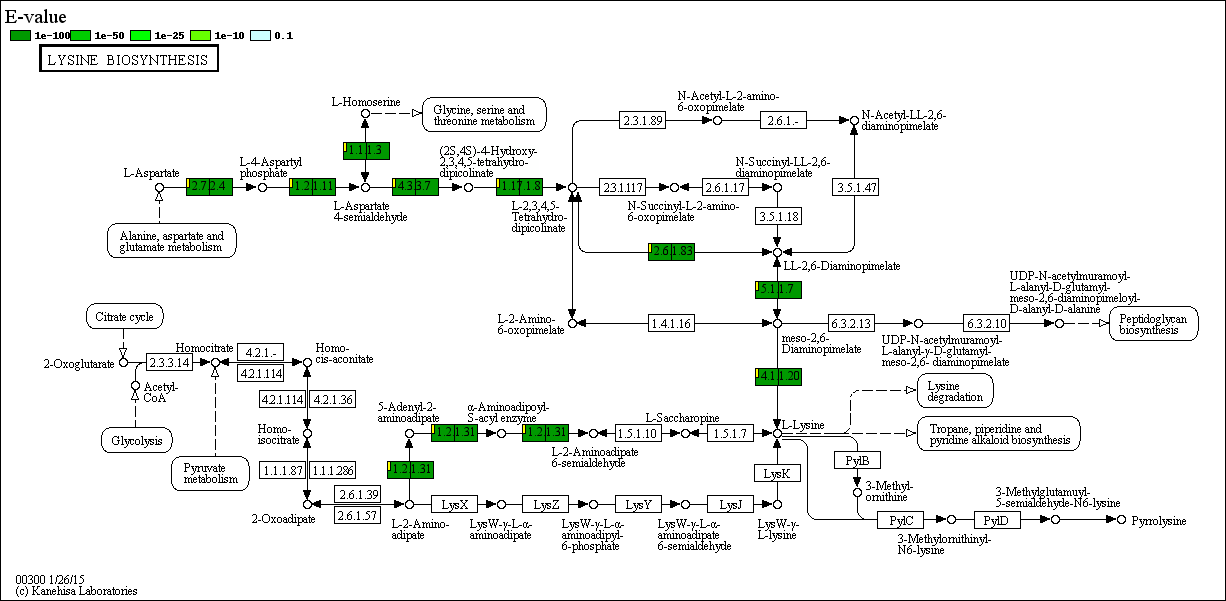
\includegraphics[width=0.8\textwidth]{map00300.png}
    \captionsetup{labelsep=period}
    \caption{QC分析结果}
\end{figure}
为便于查看差异基因在通路图中的分布情况,我们将差异基因标注到通路图中,查看方法如下:拿到全部分析结果后,打开out结果目录中文件夹下04.OtherDatabase文件夹子文件夹下的KEGG目录,解压Pathway.tar.gz压缩包,点击index.html进行浏览,您点击不同的通路名称会弹出相应的通路图。其中,蓝绿色标记代表以样本作为query,以KEGG数据库作为subject进行序列比对的结果。红黄色标记代表以KEGG作为query,以样本蛋白质序列作为sujbect进行比对的结果。比对结果的e value范围以不同颜色进行区分,如果两者blast结果形成双向最优,则在KO的节点左上角形成黄色标记。包含下鼠标悬停于标记的KO节点,弹出基因细节框,包括核酸序列,蛋白序列以及序列比对情况。以上步骤可脱机实现,如连接互联网,点击各个节点,可以连接到KEGG官方数据库进行查看。
%
%\input{ "{{kg}}"   }
%


\subsection{CDS序列多数据库比对注释}
将所有的CDS序列利用blast比对到KEGG、Swissprot、Nr、Nt、eggNOG数据库,e-value阈值统一为1e-35。结果如下:
%\input{ "{{annotationtable}}"}

%\input{ "{{annotationgraph}}"}